\chapter{Conclusions \& Musings}



\section{HHT Pathogenesis}






\section{CCM Pathogenesis}
\subsection{Regrowth after Surgical Resection}
\subsection{CCM \& Meningioma}
Although the vascular lesions are the primary sequelae of familial CCM, many groups have noted an increased prevalence of meningioma in individuals with familial CCM—especially those with a mutation in \italicize{PDCD10} \citep{labauge2009, riant2013, garaci2015}. In addition, we have previously been contacted by an individual whose child had a sporadic CCM that regrew into a meningioma. Unfortunately we were unable to acquire a tissue sample for genetic analysis, however this case along with the strong link between familial CCM and meningioma has fueled my interest in understanding the link between CCM and meningioma. 
\subsubsection{Kruppel-like factor 4 (\italicize{KLF4})}
\italicize{KLF4} is a transcription factor with key roles in the pathogenesis of both CCM and meningioma. In CCM, \italicize{KLF4} (along with \italicize{KLF2}) is a key player in CCM signaling that is upregulated by loss of the CCM complex or gain of function in \italicize{MAP3K3} \citep{cuttano2016, zhou2016}. Indeed, overexpression of \italicize{KLF4} in mouse models leads to an aggressive CCM-like phenotype \citep{ren2021}. In meningioma, mutations in \italicize{KLF4} are common and often co-occur with mutations in \italicize{TRAF7} \citep{reuss2013}. In addition, \italicize{KLF4} mutated meningioma have been shown to be responsive to treatment with temsirolimus \citep{vonSpreckelsen2020}—a derivative of rapamycin (sirolimus) which has been shown to be effective in treating CCM in mice \citep{ren2021}. The importance of \italicize{KLF4} in both CCM and meningioma suggests that dysregulation of \italicize{KLF4} may underlie the development of meningioma in individuals with familial CCM. 

The majority of \italicize{KLF4} mutations found in the catalog of somatic mutations in cancer (COSMIC) result in p.K409Q (Figure~\ref{KLF4_COSMIC}A). This narrow spectrum of mutations suggests that the p.K409Q variant results in KLF4 gain of function. Notably, the p.K409Q mutation is highly specific to meningioma, occurring in very few other cancer types (Figure~\ref{KLF4_COSMIC}B). The KLF4 protein contains 3 DNA-binding zinc-finger domains that contribute to its activity as a transcription factor. The p.K409Q mutation occurs in the first of the three zinc-finger domains (Figure~\ref{KLF4_COSMIC}C). A structural study of KLF4 determined that the second two zinc-finger domains consistently bind DNA, however the first zinc-finger only sometimes participates in DNA binding \citep{schuetz2011}. They determined that the second and third domains are required for site specificity, but the third "inhibits cryptic self-renewal and block of differentiation activity". This immediately suggests a mechanism by which the p.K409Q mutation may disrupt the inhibitory capacity of KLF4 while retaining its functions that are independent of the first zinc-finger domain. 

%%%%%%%%%%%%%%%
\begin{figure}[tbp!]
\begin{center}
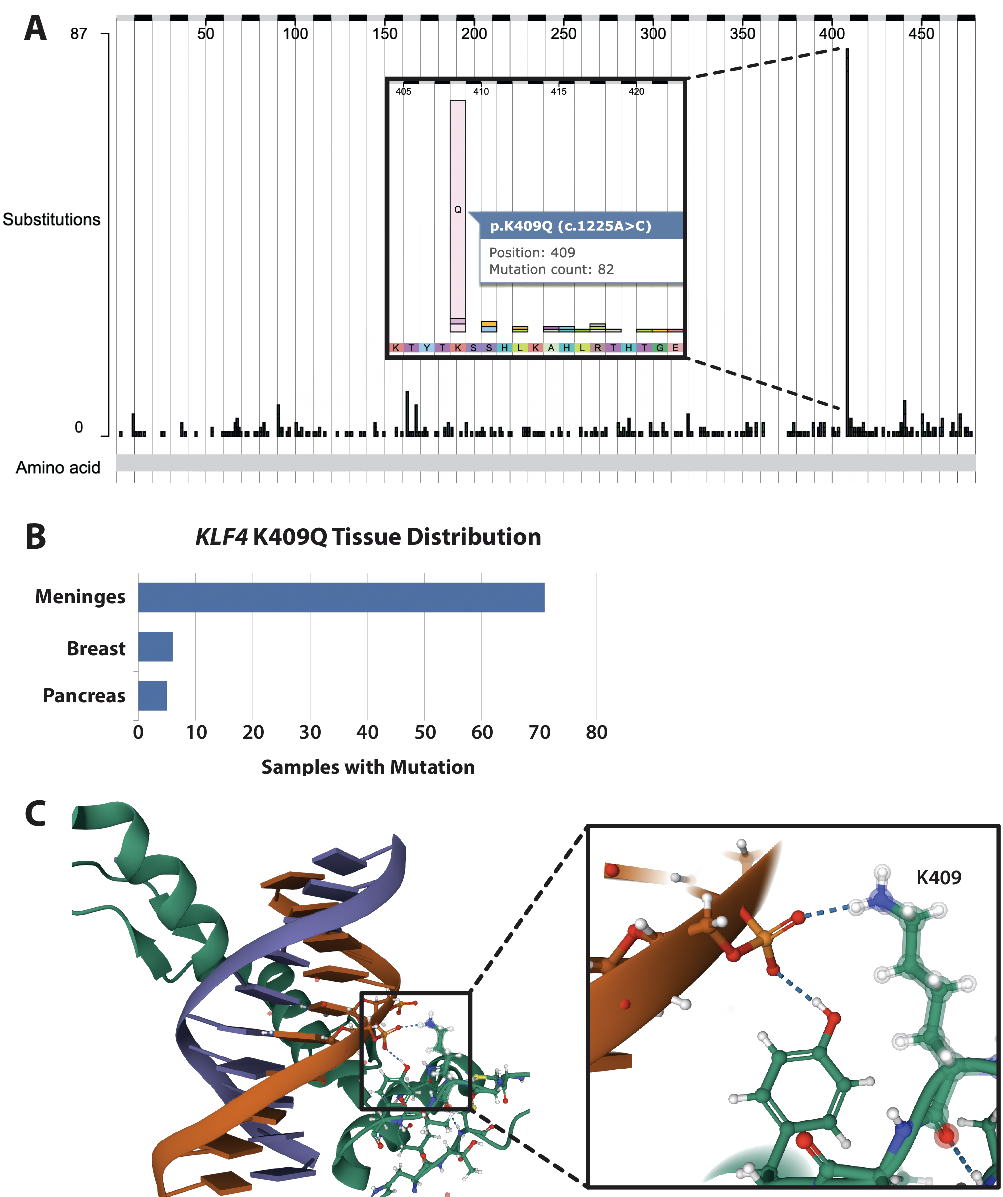
\includegraphics[width=5in]{KLF4_COSMIC}
\end{center}
\caption[\italicize{KLF4} Mutations in COSMIC]{\italicize{KLF4} Mutations in COSMIC. 

A. Distribution of somatic mutations in \italicize{KLF4} that are present in the catalog of somatic mutations in cancer (COSMIC). The location of the most frequent mutation (p.K409Q) is expanded in the inset. B. Distribution of \italicize{KLF4} p.K409Q in tissue types present in COSMIC. C. Structure of KLF4 zinc-finger domains bound to DNA (PDB: 2WBU). Border box denotes the expanded region to the right showing the interaction between K409 and the DNA backbone.}
\label{KLF4_COSMIC}
\end{figure}
%%%%%%%%%%%%%%

I though that since overexpression of \italicize{KLF4} is sufficient to cause CCM in mice, the p.K409Q mutation may cause some sporadic CCMs in humans. To test this, I developed a ddPCR assay to test for this mutation in 30 mutation-negative sporadic CCM, however I did not find evidence for this mutation in any of these samples. This may be a reflection of the highly specific functions of the first zinc-finger domain in KLF4 as discussed above. This function may be critical for meningioma development, but less important for CCM development. However, the inverse is not necessarily true—i.e.~while the p.K409Q mutation may not cause CCMs, overexpression of \italicize{KLF4} may cause meningioma. This is currently unknown, though if true, may account for the presence of meningioma in familial CCM. One straightforward way to test this hypothesis would be to sequence tissue from meningioma in individuals with familial CCM. I suspect that these meningioma harbor a somatic loss of function mutation in \italicize{KRIT1/CCM2/PDCD10} leading to biallelic loss of a CCM gene resulting in upregulation of \italicize{KLF4}. These meningioma may also harbor a second mutation in \italicize{TRAF7} which have often been found in non-CCM meningioma. Unfortunately, tissue samples of meningioma from individuals with familial CCM have been difficult to acquire, thus I have been unable to test this hypothesis. However, I expect that future studies will find that \italicize{KLF4} is a critical link between CCM and meningioma. 











\section{Developmental Venous Anomalies as a Primer for Disease}
\subsection{Association with Sporadic CCM}
\subsection{Association with Other Diseases}
\subsection{Cowden Syndrome}
\subsection{Implications}













\section{Other Vascular Malformations}
\subsection{Classification of Vascular Malformations and Vascular Tumors}

\subsection{Sturge-Weber Syndrome and Somatic Mutations in \italicize{GNAQ}}
\subsubsection{Happle's hypothesis}
\subsubsection{\italicize{GNAQ} in uveal melanoma and circumscribed choroidal hemangioma}
\subsubsection{Link between SWS, UM, and CCH?}

\subsection{The Curious Case of Infantile Hemangioma}
Infantile hemangioma (IH) are one of the most common vascular malformations. They occur in children and are typically present at birth as a red spot flush with the surrounding skin. Soon after birth the hemangioma rapidly grows and becomes raised from the skin. They are generally benign and are typically left alone unless they cover the child's mouth, nose, or eyes. What makes IH so interesting compared to other types of vascular malformations is that they almost always completely regress within the first few years of the child's life. While other types of vascular malformations may spontaneously regress (telangiectasia and AVMs), none do so with the consistency of IH. This phenomenon has been of great interest, not for the purpose of developing therapeutics for IH (propranolol is an extremely effective treatment for IH) but for uncovering the mechanism of regression in the hopes that what we learn can be applied to regress other, more nefarious, vascular malformations. 

\subsubsection{GLUT1 in IH endothelium}
Perhaps one of the most provocative discoveries into the mechanism of IH pathogenesis is the fact that endothelial cells from IHs highly express GLUT1 \citep{north2000, north2001}. GLUT1 is a glucose transporter that has remarkable specificity for the placental endothelium. This finding suggested that the IH may be comprised of cells that dislodged from the maternal placenta, then became hyper-proliferative in a post-fetal environment. If this hypothesis is correct, one would expect to find that the IH is a genetically chimeric growth between fetal and maternal cells. This hypothesis was put to the test using fluorescence \italicize{in situ} hybridization to assay the presence of XX cells in IH from a male infant with confirmation by sequencing microsatellites and SNPs that were divergent between mother and child. This analysis found no evidence for maternal-fetal chimerism in IH \citep{pittman2006}. Despite this counter-evidence, the presence of GLUT1 in IH is strongly indicative of some link with the placenta though unfortunately this link currently remains elusive. The current literature has very clearly shown the presence of GLUT1 in IH endothelial cells, however the extent of the placental transcriptional program is unclear. Epigenomic profiling of paired IH and maternal placental samples may give valuable insights into the mechanism of IH. 

\subsubsection{Efforts to find somatic mutations in IH}
As it is quickly becoming clear that the vast majority of vascular malformations are the result of somatic mutations—many occurring in known oncogenes—I thought that somatic mutations may also underlie IH. To test this, I sequenced 61 IH lesions on an 'oncopanel' covering many genes that are highly mutated in cancers as well as several genes previously implicated in vascular malformations (\italicize{KRIT1, CCM2, PDCD10, ACVRL1, ENG, SMAD4,} etc.) Unfortunately after filtering putative variants, no there were no variants with likely functional significance and that occurred in more than a single sample. I am aware of at least 1 other group that has attempted to identify somatic mutations in IH via whole-exome sequencing, however to date there are no known somatic mutations in IH. One important aspect of these studies that must be noted is that they are invariably focused on coding regions of the genome. Non-coding variants are more than capable of causing disease however discovery-focused sequencing studies often ignore non-coding regions both because of the cost of sequencing the entire genome to a depth sufficient to detect somatic mutations, and the challenges associated with functional analysis of non-coding variants. Further studies may find that somatic mutations do cause IH, but they occur in a region of the genome that is missed by the majority of sequencing studies. 









\section{The Molecular Basis of Genetic Dominance}
\subsection{Phenotypic Dominance $\neq$ Genetic Dominance}
\subsection{Knudsons Fingerprint}
\subsection{The Diverse Functional Effects of Genetic Mutations}










\section{The Intersection of Somatic Mutagenesis and Evolution}
\subsection{The Creation of New Alleles}
\subsection{The Relationship Between Mutability and Fitness Landscape}
\subsection{Recurring Mutations \& Convergent Evolution}
\subsection{Clonal Evolution of Somatic Mutants}
\subsection{Cancer}










\section{Somatic Mutations}
\subsection{The Role of Somatic Mutations in Aging}
\subsection{Constitutional Intolerance \& Somatic Permissiveness}
\subsection{Somatic Reversion of Pathogenic Mutations}
\subsection{What is the Consequence of RNA Mutations?} 
%mutations at the RNA level i.e. individual mutant RNA molecules
%interactions with the ribosome?
%could a single RNA molecule screw things up?









\section{Innovation in the Sequencing Era}
\subsection{Detection of Somatic Mutations}
\subsection{Single Cell Sequencing}
\subsection{Utility of Rare Disease Research in Mechanistic Discovery}
\subsection{Data Democratization \& Individual Privacy}
\subsection{Growing Importance of Informatics in Biology}